\section{Az egész rendszer architektúra}
\label{sec:rendterv}

Az egész rendszer tervezésénél első lépésben összeállítottunk rendszerünk felépítéséről egy olyan listát ahol megjelennek a fő komponenseink. Az \ref{fig:systemArchBig} ábrán látható ezeknek a komponenseknek az összesége. Megfigyelhetjük az ábrán, hogy nem a csak az elemek vannak rajta feltüntetve, hanem az elemek közötti kapcsolatok is megjelennek.
\begin{figure}[H]
	\centering
	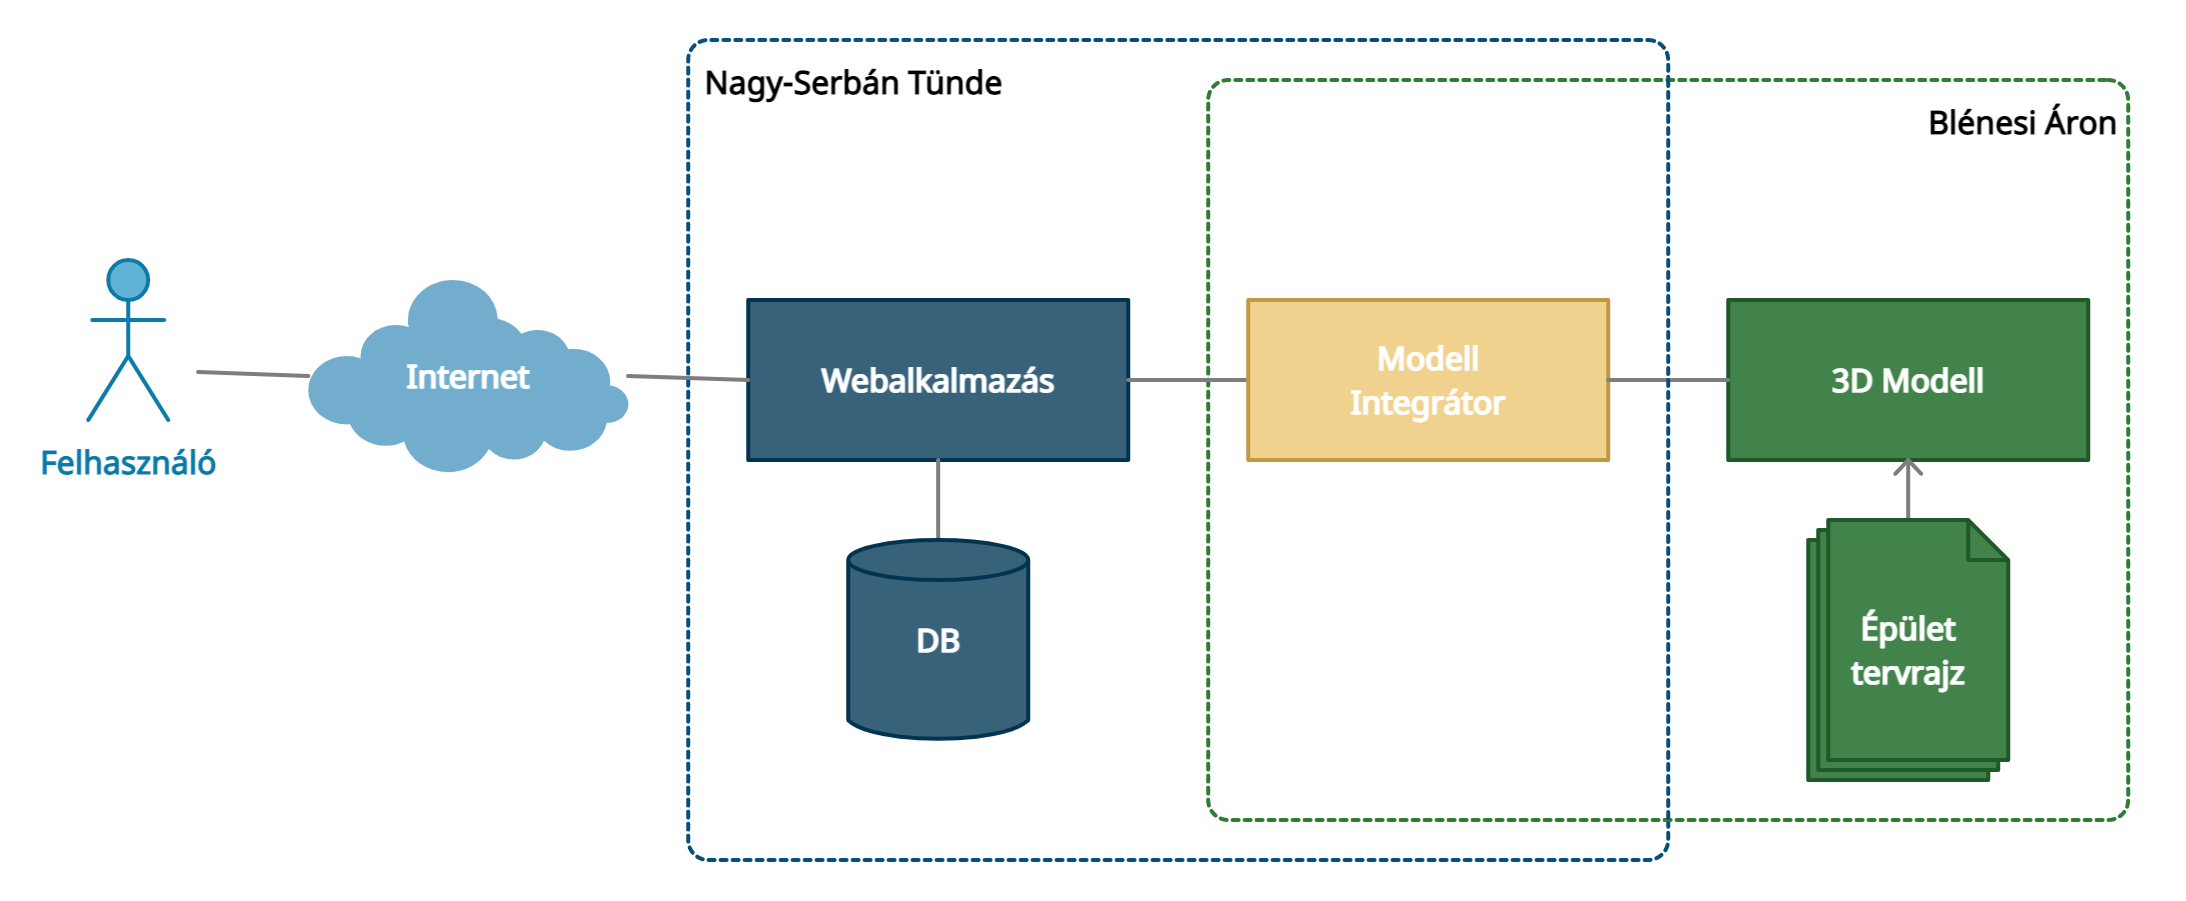
\includegraphics[width=1\linewidth]{figures/images/kozosfazis.png}
	\caption[Az egész rendszer architektúrája]{\textit{Az egész rendszer architektúrája}}
	\label{fig:systemArchBig}
\end{figure}

Amiután megszületett ez a lista rájöttünk, hogy a rendszert két részre fogjuk osztani. A 3D modell tervezését, implementálását a kollégám, Blénesi Áron készíti el míg az webalkalmazást, adatbázis tervezést én. A két a projektet egy komponensen keresztül kötjük össze. Ez a komponens a web alkalmazáson belül van létrehozva, és általa jelenítődik meg a 3D modell.

Az \ref{fig:systemArchBig} ábrán látható színeknek is megvan a maga jelentősége. A világos kék színnel látható a Felhasználó és az Internet. Ez a két komponens bíztosítja a rendszer elérhetőségét és felhasználását, mivel az interneten keresztül érik el majd a felhasználók a weboldalt, ami által használatba tudják venni a rendszert.

A sötét kék színnel jelelöltük a Webalkalamzást és az adatbázist (DB). Ezen kopmonensekről a további fejezetekben lesz szó bővebben. A sötét zöld szín a 3D modell felépítésére vonatkozik, amelyről egy másik dolgozat keretén belül lehet olvasni. (Blénesi Áron: Sapi3D tour - 3D modell). A narancssárga színnel jelölt rész lenne a két alrendszer összekötésének komponense, amelyről részletesebben lehet olvasni ezen dolgoozat további fejezeteiben és a már említett kolléga dolgozatában is.

Az egész rendszer tervezésének befejezésekor kezdődött el az alrendszerek tervezésének fázisai. A Webalkalamazás és Adatbázis tervezéséről \ref{sec:webterv} alfejezetben olvashatunk.